%%%%%%%%%%%%%%%%%%%%%%%%%%%%%%%%%%%%%%%%%%%%%%%%%%%%%%%%%%%%%%%%%%%%%%%%%%%

\documentclass{standalone}

\usepackage{amsmath}
\usepackage{mathptmx}
\usepackage{pgfplots}
\usetikzlibrary{external}
\tikzexternalize{cricket-run-rmse}
\pgfplotsset{compat=1.16}

%% IEEE uses Times Roman font, so we'll default to Times.
%% These three commands make up the entire times.sty package.
\renewcommand{\rmdefault}{ptm}
\renewcommand{\ttdefault}{pcr}
\normalfont\selectfont

\begin{document}

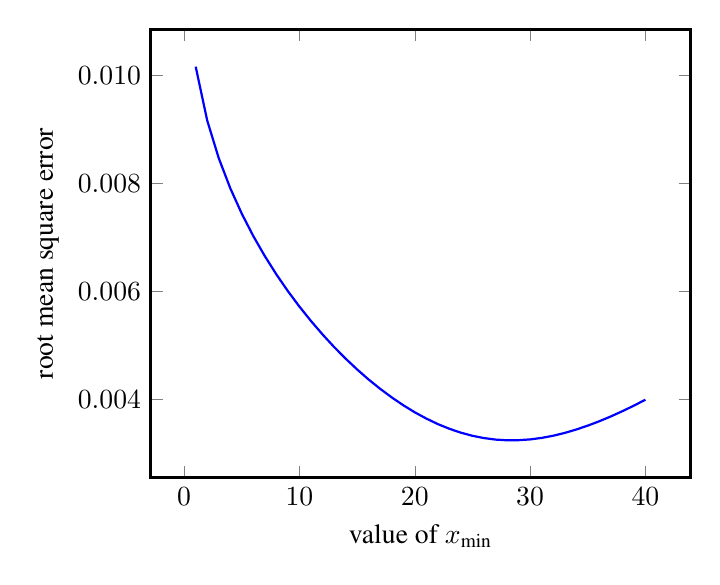
\begin{tikzpicture}
\tikzset{%%
  every mark/.append style={scale=1.0},%%
  scale=1.0%%
}
\pgfplotsset{%%
  every axis/.append style={font=\normalsize}%%
}
%%
\begin{axis}[%%
  axis line style=very thick,%%
  dotStyle/.style={blue,mark=none,thick},%%
  enlargelimits=true,%%
  %% x axis
  xlabel={\normalsize value of $x_{\text{min}}$},%%
  %% y axis
  ylabel={\normalsize root mean square error},%%
  scaled y ticks=false,%%
  ytick={0.004,0.006,0.008,0.010},%%
  yticklabels={$0.004$,$0.006$,$0.008$,$0.010$}%%
]
%%
%%
\addplot[dotStyle] coordinates {
  (1, 0.010163)
  (2, 0.009166)
  (3, 0.008470)
  (4, 0.007913)
  (5, 0.007441)
  (6, 0.007027)
  (7, 0.006656)
  (8, 0.006318)
  (9, 0.006008)
  (10, 0.005722)
  (11, 0.005456)
  (12, 0.005208)
  (13, 0.004976)
  (14, 0.004761)
  (15, 0.004560)
  (16, 0.004373)
  (17, 0.004201)
  (18, 0.004043)
  (19, 0.003898)
  (20, 0.003767)
  (21, 0.003651)
  (22, 0.003549)
  (23, 0.003462)
  (24, 0.003390)
  (25, 0.003332)
  (26, 0.003290)
  (27, 0.003262)
  (28, 0.003249)
  (29, 0.003251)
  (30, 0.003265)
  (31, 0.003293)
  (32, 0.003333)
  (33, 0.003385)
  (34, 0.003448)
  (35, 0.003520)
  (36, 0.003601)
  (37, 0.003690)
  (38, 0.003787)
  (39, 0.003890)
  (40, 0.004000)
};
\end{axis}
\end{tikzpicture}

\end{document}
